\documentclass{article} % For LaTeX2e
\usepackage{nips13submit_e,times}
\usepackage{graphicx}
\usepackage{hyperref}
\usepackage{url}
%\documentstyle[nips13submit_09,times,art10]{article} % For LaTeX 2.09


\title{Localizing a SCUBA Diver Using Active Sonar}


\author{
Richard Guilmain \\
Georgia Institute of Technology\\
\texttt{richguilmain@gatech.edu} \\
\And
Nabin Sharma \\
Georgia Institute of Technology\\
\texttt{nsharma@gatech.edu} \\
}

% The \author macro works with any number of authors. There are two commands
% used to separate the names and addresses of multiple authors: \And and \AND.
%
% Using \And between authors leaves it to \LaTeX{} to determine where to break
% the lines. Using \AND forces a linebreak at that point. So, if \LaTeX{}
% puts 3 of 4 authors names on the first line, and the last on the second
% line, try using \AND instead of \And before the third author name.

\newcommand{\fix}{\marginpar{FIX}}
\newcommand{\new}{\marginpar{NEW}}

\nipsfinalcopy % Uncomment for camera-ready version

\begin{document}


\maketitle

%% \begin{abstract}
%% \end{abstract}

\section{Problem Description}
The threat of an underwater terrorist attack is a concern of the maritime industry, port law enforcement, and luxury and high-profile vessel owners alike. Prevention of such attacks needs to start with the reliable detection of sub-surface threats such as SCUBA and closed-circuit re-breather (CCR) divers. Because these threats are below the water's surface, traditional detection methods such as radar and visual surveillance are unavailable. This makes active sonar technology the most effective approach to date. However, because of the inherent noise of the underwater acoustic environment\textemdash often rife with mechanical noise, reflective debris, and environmental marine activity\textemdash current sonar methods are often inconsistent. Underwater targets like SCUBA divers might not be detected at all measurement steps even if relatively noisier measurements are accepted as valid ones. This leads to the requirement of more robust localization schemes so that we don't lose valid targets. Better processing methods are required to manage this low signal-to-noise ratio while still localizing the range and bearing of threatening divers at tactically significant ranges.

\begin{figure}[htbp]
  \centering
  \fbox{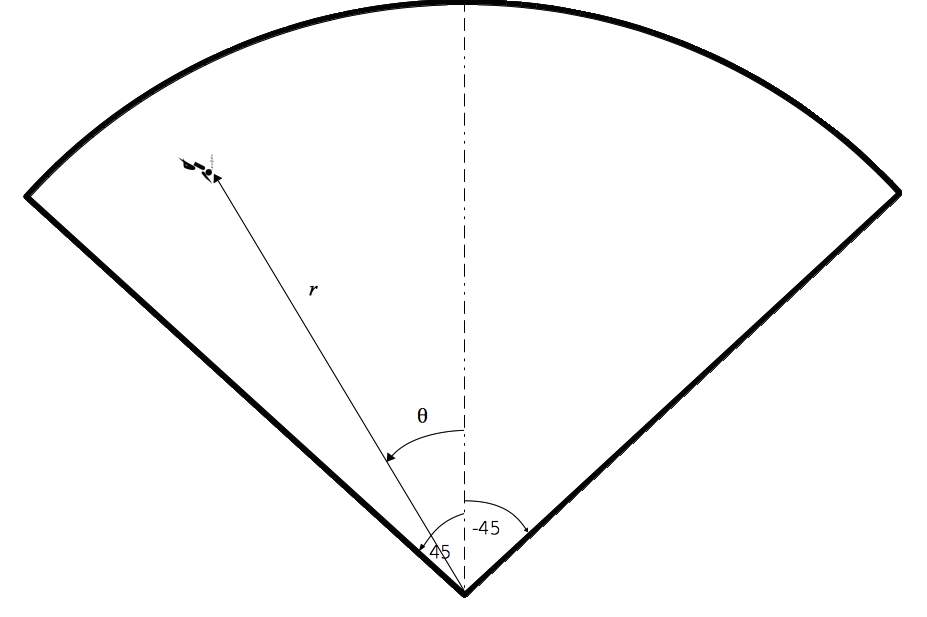
\includegraphics[width=0.9\textwidth]{sector.png}}
  \caption{Basic graphical representation of a typical diver localization scenario. Sonar
    measurements provide the range ($r$) of the target (or diver) from the sonar sensor and
    bearing ($\theta$) from the sonar sensor axis represented by a dashed line. The angular
    span of the sensor field-of-view is $90^{\circ}$.}
  \label{fig:sector}
\end{figure}

\section{Sensor and Measurements}
Figure \ref{fig:sector} shows a typical diver localization scenario. The bottom center point of the sector in Fig.~\ref{fig:sector} represents the location of an active sonar sensor located either on a fixed platform (such as a pier) or on a rotating and translating platform (such as an anchored vessel). In the case of a moving platform, a GPS device and a heading sensor are also used at this point to track the sonar's motion.
The sonar is capable of detecting targets within 500 meters and up to 45 degrees on either side of a direct forward line-of-sight. The sonar transmits an acoustic pulse every 1.3 seconds and listens for echo returns via a multichannel receive array.

Figure \ref{fig:blocks} shows the signal and data processing block diagram of the sonar system. Data received from the sensor array passes through several signal processing modules, including a lowpass filter and a digital downconverter, before it gets beamformed.

\begin{figure}[htbp]
  \centering
  \fbox{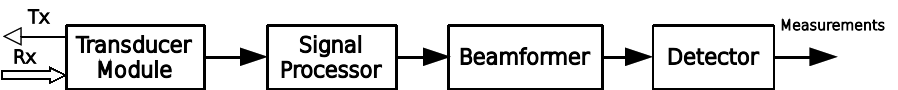
\includegraphics[width=0.9\textwidth]{blocks.png}}
  \caption{Block diagram of the active sonar receiver used to obtain diver measurements.}
  \label{fig:blocks}
\end{figure}

During beamforming, the sonar software combines the signals from all of the receiving array channels in a controlled manner such that the time delays experienced by the sonar echoes are equalized for desired directions. This effectively increases the receiver gain in the desired directions and thus helps to get better target measurements. An example output from the beamformer is shown in Fig.~\ref{fig:sector_example}.

\begin{figure}[htbp]
  \centering
  \fbox{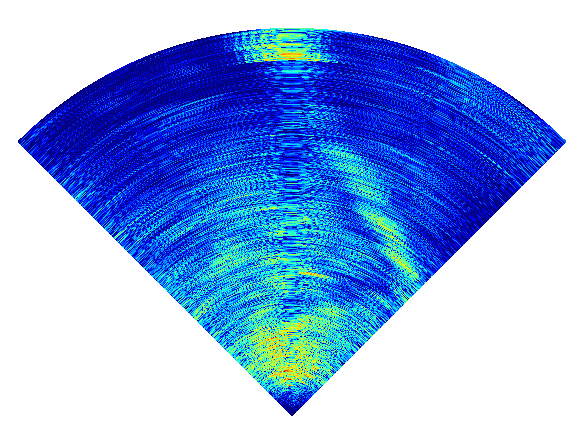
\includegraphics[width=0.9\textwidth]{sector_example.png}}
  \caption{A representative sonar sector. The relatively stronger patch at around $0^{\circ}$ and 450 meters is a diver.}
  \label{fig:sector_example}
\end{figure}

After beamforming, the sonar software detects areas of high signal return. The detector attempts to minimize the effects of noise and false detections as much as possible without losing the true target measurements. To do this, it implements ping-to-ping exponential smoothing and background subtraction algorithms to provide relatively cleaner moving target measurements to the localization algorithm. The targets that are of most importance are the ones moving toward the sonar (a diver traveling away from us isn't nearly as much of a potential threat as one swimming toward us). Therefore, the detector is tuned to detect targets that are moving radially towards the sonar sensor more effectively than targets moving otherwise.

It is evident from Fig.~\ref{fig:sector_example} that the sector data coming out of the beamformer can be quite noisy depending on the conditions of the water and the surrounding environment. As such, we have to accept some level of false detections to also pick up on true measurements of the diver. This leads to the requirement of a probabilistic localization algorithm if we want to detect the diver with a high level of confidence.

\section{Hypothesis and Project Approach}
We believe that a good solution to this problem of diver localization in an inherently noisy environment is to make use of a particle filter. Particle filters are a robust solution because they can handle the entropy associated with sensor error and the inexact motion of both the diver and the platform that the sensor is mounted on.
Other options included using a histogram filter, which we decided against because we are working in a continuous environment, and using a Kalman filter, which we decided against because we did not want to assume a uni-modal distribution (there could be more than one threat in the water) and because we were unconcerned with scaling past two dimensions.

\section{Implementation Details}
Because the sonar may be mounted on a moving platform, we used the GPS and heading information located at the sensor to update our expectation of the relative distance and bearing to our particles over time. The particle filter algorithm starts by initializing a pool of particles at random range and horizontal angles within the field-of-view. Then, at every ping (i.e. transmit/receive cycle), it updates the position of the particles relative to how the sensor (sonar) moved and translated. The prediction step introduces some randomness into the range ($r$) and horizontal angle ($\theta$) of the particle according to
\begin{eqnarray*}
  r_{new} = r_{old} + n_r \\
  \theta_{new} = \theta_{old} + n_{\theta},
\end{eqnarray*}
where $n_r$ and $n_{\theta}$, representing range noise and angle noise, respectively, are Gaussian random variables with zero mean. The variance of these noises are determined by the accuracy of the sonar detector. Typical values for $n_r$ and $n_{\theta}$ are 3 meters and 3 degrees, respectively.

After sensor motion is accounted for, the filter does a weighted resampling with replacement of the particles with a Gaussian bias toward resampling points that are close in range and horizontal angle to the measurements outputted by the detector as shown in Fig.~\ref{fig:blocks}.

After the measurement update, the estimated diver position is computed as the mean of the positions of all of the particles.

\begin{figure}[htpb]
  \centering
  \fbox{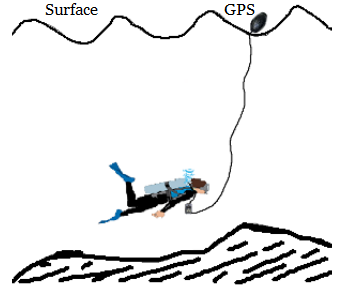
\includegraphics[width=0.6\textwidth]{diver_gps_setup.png}}
  \caption{Diver GPS setup to collect approximate ground truth.}
  \label{fig:diver_gps_setup}
\end{figure}

\section{Analysis of Results}
During the data collection, our diver was connected to a GPS device floating on the water's surface by a 25 meter long tether as shown in Fig.~\ref{fig:diver_gps_setup}. Because of drifting, the GPS was never directly above the diver. As such, it does not provide us with an exact location of where the diver was, but it does provide a useful envelope of error metric with which we can evaluate the output of our particle filter.

Figure \ref{fig:particle_532} shows an intermediate result from our particle filter while a diver approaches the sonar. The cloud of blue dots represents the current set of particles, the red dots represent the current measurements from the sonar detector, and the cyan colored dot-dash curve is the accumulated history of diver position estimates.

For the first dozen or so pings at the the start of the localization, there are many noisy detections in the field-of-view, and the particles do not converge on any one in particular. As a result, the estimated diver location moves around quite a bit. However, since the diver is the most consistent of the detections, the particles migrate away from the transient false positives and toward the stable true positive. By the time the diver reaches about 350 meters from the sonar, the particles converge, and generally ignore transient false detections that appear far away from the diver.

Figure \ref{fig:track_vs_diver_gps} shows the diver track estimated by our filter and the approximate ground truth of the diver as determined by the diver GPS. Once the particles converge, the calculated diver position follows very closely to the approximate output from the GPS. In fact, it often follows within just a few meters of the GPS floating at the water's surface, well within our envelope of error.

\begin{figure}[htbp]
  \centering
  \fbox{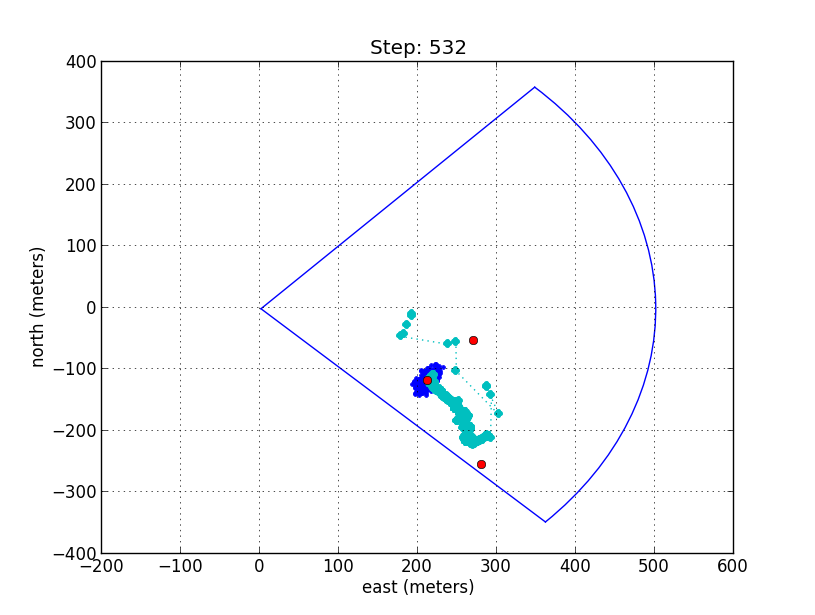
\includegraphics[width=0.8\textwidth]{particle_532}}
  \caption{Diver localization using a particle filter. Blue dots represent
    the particles, red dots are the current measurements, and the cyan curve is
    the estimated diver track. The diver is moving toward the sensor.}
  \label{fig:particle_532}
\end{figure}

It is important to note that during a diver attack, the quicker you can detect the attacker, the quicker you can respond. The fact that this filter was able to lock on to the correct target in fewer than 15 pings (less than 20 seconds) suggests that this approach could not only be feasible, but it could also be very useful.

\begin{figure}[htbp]
  \centering
  \fbox{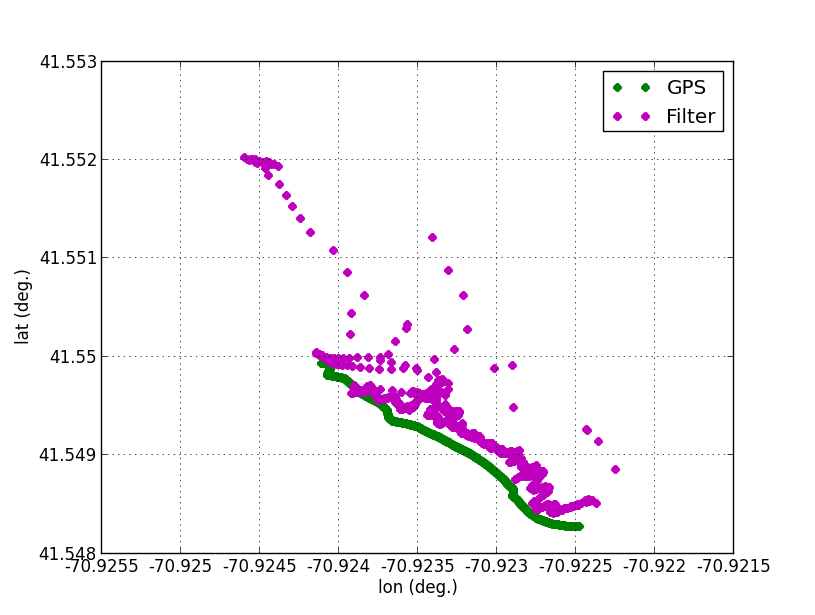
\includegraphics[width=0.8\textwidth]{track_vs_diver_gps.png}}
  \caption{Comparison of the diver track from our particle filter plotted
    alongside the approximate ground truth received from the diver GPS.}
  \label{fig:track_vs_diver_gps}
\end{figure}

\section{Future Work}
Currently, we calculate the position of the diver as the mean of the particle positions. However, because our particle filter is multi-modal, it is can (and often does) find multiple targets. One way of picking up on this behavior would be to first perform distribution-based clustering of the particles to determine how many in-water target clusters there are. Then, we could find the center of each cluster and create multiple tracks. Expectation-Maximization would be a strong candidate for our clustering algorithm because it assumes an underlying Gaussian cluster structure. Because of how our particle filter takes motion and measurement noise into account, our clusters are guaranteed to be Gaussian.

Also, in addition to localizing divers' positions, we could also find their speeds and headings. This is possible because we have data from them over many iterations. This extra information could be useful for providing such features as predicted paths and estimated times of arrival of the targets. Additionally, because different kinds of targets have different speeds\textemdash a human diver versus debris being carried by the current versus marine life type A versus marine life type B, for example\textemdash this extra information would be valuable for performing target classification.

\section{Conclusion}
We have shown that active sonar paired with a particle filter can be effective in localizing underwater threats such as SCUBA and CCR divers, even from non-stationary platforms. Furthermore, we showed that the use of a probabilistic approach to diver localization has the benefit of being robust to measurement and motion noise. We also stated several approaches that future research can take to further increase the awareness of defense organization such as governmental port law enforcement.

\section*{YouTube Link of Video Presentation}
\url{http://youtu.be/SxWdn8NxcE8}

\end{document}
